\chapter[Test Driven Development]{Test Driven Development}
  \section{Czym jest TDD?}
    Test Driven Development jest praktyką, według założeń której każda modyfikacja systemu poprzedzona jest stworzeniem odpowiedniego testu opisującego tą modyfikację. Programista zaczyna od napisania testu, który z naturalnych przyczyn (testowany kod nie istnieje a tym etapie) daje wynik negatywny. Następnie napisany zostaje właściwy kod, którego zachowanie zgodne jest z testowanym. Kiedy testy przechodzą można wprowadzić ewentualne poprawki.
    Proces rozwoju oprogramowania w zgodzie z filozofią TDD składa się z wielu takich cyklów, które zobrazować można diagramem:
    
    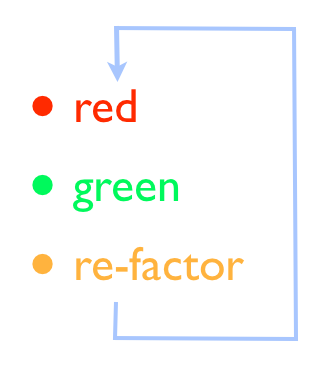
\includegraphics[width=75mm]{images/tdd_red_green_refactor.png}
    
    \begin{description}
      \item[Red] Pierwszy etap cyklu otrzymał swoją nazwę ze względu na to, że w większości środowisk służących do testowania oprogramowania testy, które zakończyły się niepowodzeniem oznaczane są czerwony kolorem. Etap ten polega na napisaniu testu przed rozpoczęciem implementacji właściwej funkcjonalności oraz na uruchomieniu go. Należy upewnić się, że w tym momencie test zakończy się niepowodzeniem - daje to pewność, że faktycznie testujemy nowe zachowanie, którego w tym momencie system jeszcze nie obsługuje a także że ewentualna przypadkowa modyfikacja tego zachowania zawsze zostanie wykryta przez nieprzechodzący test.
      \item[Green] Drugi etap polega na zaprogramowaniu zachowania opisanego wcześniejszym testem. Programista piszę tylko tyle kodu, aby spełnić warunki testu po czym uruchamia ponownie cały zestaw testów. Uruchomienie tylko ostatniego testu związanego z napisanym kodem jest nie wystarczające - może okazać się, że nasze ostatnie zmiany modyfikują bezpośrednio lub pośrednio wiele obszarów aplikacji. Jak wskazuje nazwa, etap ten powinien zakończyć się gdy wszystkie do tej pory stworzone testy przechodzą pozytywnie.
      \item[Re-factor] Ostatni etap polega na jakościowej modyfikacji kody. W tym momencie programista powinien skupić się na usunięciu wszelkich zbędnych powtórzeń, uproszczeniu implementacji czy też dopracowaniu użytego nazewnictwa zmiennych lub metod. Etap ten nie pociąga za sobą żadnych zmian w sposobie działania oprogramowania, jest jednak równie ważny jak poprzednie, dobry jakościowo kod jest łatwiejszy w utrzymaniu i modyfikacji.
    \end{description}
    
    Opisane powyżej iterację powinny być jak najprostsze. Oznacza to, że każdą implementowaną funkcjonalność należy podzielić na jak najmniejsze części i wykonywać pełen zestaw powyższych kroków dla każdej z nich. Idealna sytuacja to taka, w której pojedynczy test sprawdza tylko jedną rzecz.

  \subsection{Główne zasady TDD}
    \paragraph{Zacznij od testu}
      Test powinien być napisany zanim zacznie się implementacja funkcjonalności. Takie podejście gwarantuje, że będziemy mieli pełen zestaw testów opisujących każdą funkcję systemu. Inną zaletą jest konieczność dokładnego przemyślenia szczegółów implementacji jeszcze przed jej rozpoczęciem.
    \paragraph{Zaraz po napisaniu nowe testy powinny dawać negatywny wynik}
      Daje to pewność, że testy faktycznie spełniają swoją funkcję, oraz każda degradacja funkcjonalności będzie sygnalizowana nieprzechodzącym testem.
      
  \subsection{Przykładowe iteracja TDD}
    Przypuśćmy, że pracujemy nad oprogramowaniem sportowej tablicy wyników. Naszym aktualnym zadaniem jest napisanie metody, która na wejściu otrzymuje nazwy dwóch drużyn sportowych, zwraca zaś łańcuch składający się z nazw tych drużyn połączonych łańcuchem " vs ". Oprogramowanie napisane jest w języku Ruby, do testowania użyjemy biblioteki RSpec.
    
    Praca rozpoczyna się od napisania testu opisującego pożądane zachowanie. W naszym wypadku może on wyglądać tak: 
    
    \lstinputlisting[language=ruby]{examples/code/ch02/01.rb}

    Dokładny opis budowy testu zawarty jest w podrozdziale 'Narzędzia wspierające TDD dostępne dla języka Ruby' i nie będę go tutaj powielał. Chciałbym jednak zwrócić uwagę na fakt, że już na etapie pisania testu programista zmuszony jest przemyśleć szczegóły implementacji. Zaprezentowany przykład jest bardzo prosty, ale na pierwszy rzut oka widać, że oprócz sprawdzenia poprawności zwracanego wyniku test definiuje także pewne szczegóły architektury programu. Po pierwsze zakładamy, że tablica wyników reprezentowana będzie przez klasę o nazwie \verb+SportsTable+, a żądana funkcjonalność zostanie zaimplementowana jako metoda instancyjna \verb+header+ a więc aby mieć z niej pożytek użytkownik musi skorzystać z istniejącego obiektu tej klasy. Widać tutaj wyraźnie jedną z głównych zalet testowo zorientowanych metodyk rozwoju oprogramowania - konieczność dokładnego przemyślenia szczegółów implementacji przed jej rozpoczęciem.
    
    Sednem tego konkretnego testu jest jednak upewnienie się, że dla przykładowych danych wejściowych otrzymamy poprawny wynik. W tym wypadku sprawdzamy, czy wywołanie metody 
    
    \begin{lstlisting} 
      header('Chicago Bulls', 'Los Angeles Lakers')
    \end{lstlisting}
    
    na obiekcie klasy \verb+SportsTable+ zwróci łańcuch znaków:
    
    \begin{lstlisting} 
      Chicago Bulls vs. Los Angeles Lakers
    \end{lstlisting}
    
    Po napisaniu uruchamiamy nasz zestaw testów, co kończy się porażką. Zakładając, że rozpoczęliśmy pracę z istniejącą, pustą definicją klasy \verb+SportsTable+ zdefiniowaną w pliku \verb+sports_table.rb+ wynik powinien wyglądać następująco:

    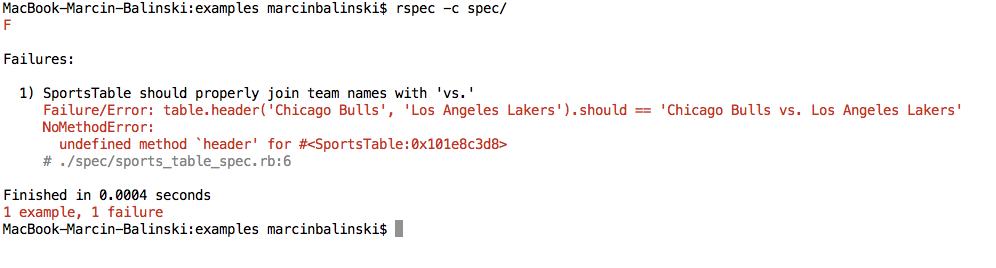
\includegraphics[width=160mm]{images/example1_failure.png}
    
    Tym samym zakończyliśmy pierwszy etap: opisaliśmy wymagane zachowanie testem oraz upewniliśmy się, że test nie przechodzi. Następnym krokiem jest napisanie pierwszej wersji metody \verb+header+:
    
    \lstinputlisting[language=ruby]{examples/code/ch02/02.rb}
    
    Ponowne uruchomienie zestawu testów kończy się sukcesem:
    
    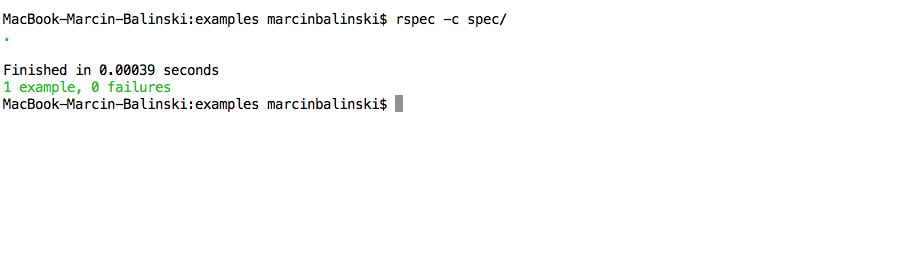
\includegraphics[width=160mm]{images/example1_success.png}
    
    Nasza metoda spełnia wszystkie założenia opisane przez testy, wciąż jednak jest pole do poprawy jakości kodu. W języku Ruby każda metoda domyślnie zwraca ostatnią zdefiniowaną w swoim ciele wartość, możemy więc zrezygnować ze zbędnego słowa kluczowego \verb+return+. Oprócz tego zmienimy sposób konstrukcji wynikowego łańcucha: zrezygnujemy z operatora \verb+++ na rzecz metody \verb+join+ obiektu klasy \verb+Array+. Po modyfikacji metoda \verb+header+ wygląda następująco:
    
    \lstinputlisting[language=ruby]{examples/code/ch02/03.rb}
    
  Powtórne uruchomienie zestawu testów kończy się sukcesem, a pierwsza iteracja TDD jest zakończona. Zdołaliśmy opisać nową funkcjonalność oraz poprawnie ją zaimplementować. W tym miejscu należy dodać, że w trzecim kroku, po modyfikacji i ulepszeniu kodu nie zmodyfikowaliśmy zestawu testów. W tym konkretnym przypadku najważniejszy dla nas jest wynik działania metody \verb+header+, nie zaś szczegóły implementacji. Nie testujemy np. tego, że konstrukcja wynikowego łańcucha znaków odbywa się z użyciem metody \verb+join+. Czasami jednak szczegóły implementacji są równie ważne jak zwracane wynik i wtedy należy napisać odpowiednie testy.
    
  \subsection{Zalety TDD}
    Test Driven Development wymusza na programiście konkretną dyscyplinę pracy. Proces rozwoju oprogramowania jest iteracyjny i bardzo uporządkowany a także wymaga uprzedniego zaplanowania każdej zmiany lub dodatku do istniejącej bazy kodu. Każda iteracja może zostać zakończona jedynie, gdy wszystkie testy zakończą się sukcesem. Taki sposób pracy niesie ze sobą wiele zalet, między innymi:
     
    \begin{itemize}
      \item Pewność, że oprogramowanie zawsze działa zgodnie z założeniami
      \item Wzrost produktywności
      \item Wzrost jakości kodu
      \item Minimalizacja liczby defektów
      \item Możliwość wczesnego wykrycia defektów
      \item Modularyzacja kodu jako pozytywny skutek uboczny
    \end{itemize}

  \section{Narzędzia wspierające TDD dostępne dla języka Ruby}
    
    \subsection{Test::Unit}
    
    Test::Unit należy do bibliotek dołączanych standardowo do każdej dystrybucji języka Ruby. Oprogramowanie testujemy tutaj przy pomocy tak zwanych asercji. Najprostsza asercja ma postać wywołania metody \verb+assert+, która sygnalizuje niepowodzenie testu w momencie, kiedy wyrażenie przekazane jako jej parametr jest fałszem, przykładowo:
    
    \lstinputlisting[language=ruby]{examples/code/ch02/04.rb}
     
     \subsubsection{Konstrukcja zestawu testów}
     Zestaw testów biblioteki Test::Unit ma postać definicji klasy, która dziedziczy po klasie Test::Unit::TestCase. Pojedyncze testy definiujemy jako metody, rozpoczynające się od ciągu znaków 'test'. W ciele każdej z takich metod możemy zdefiniować wiele asercji (aczkolwiek idealnie jest, jeśli jeden test równoznaczny jest z jedną asercją). Test kończy się sukcesem jedynie, kiedy wszystkie należące do niego asercję również zakończą się sukcesem.
     
     Przykładowy prosty zestaw testów opisujących zachowanie aplikacji będącej kalkulatorem może wyglądać tak:
     
     \lstinputlisting[language=ruby]{examples/code/ch02/05.rb}
     
     Oprócz metody \verb+assert+ biblioteka oferuje bardziej wyspecjalizowane typy asercji:
     
     \begin{description}
       \item[assert\_equal(expected, actual)] przyjmuje dwa parametry, zwraca prawdę, jeśli parametry są sobie równe.
       \item[assert\_not\_equal(expected, astual)] przyjmuje dwa parametry, zwraca prawdę, jeśli parametry różne od siebie.
       \item[assert\_match(regex, string)] przyjmuje dwa parametry w postaci łańcucha znaków lub wyrażenia regularnego, zwraca prawdę jeśli nastąpi dopasowanie wzorca.
       \item[assert\_no\_match(regex, string)] przyjmuje dwa parametry w postaci łańcucha znaków lub wyrażenia regularnego, zwraca prawdę jeśli dopasowanie wzorca nie nastąpi.
       \item[assert\_nil(object)] zwraca prawdę jeśli przekazany parametry ma pustą wartość (\verb+nil+).
       \item[assert\_not\_nil(object)] zwraca prawdę, jeśli przekazany parametr ma niepustą wartość (różną od \verb+nil+).
       \item[assert\_instance\_of(class, object)] przyjmuje na wejściu nazwę klasy oraz parametr, zwraca prawdę, jeśli parametr jest obiektem typu \verb+class+.
    \end{description}
    
    \subsubsection{Warunki początkowe i końcowe}
    Czasem grupa testów powinna być uruchamiana przy takich samych warunkach początkowych, albo też (nie tak częsty przypadek) występuje konieczność wykonania jakichś czynności na koniec każdego testu (np. wyczyszczenie bazy danych). Biblioteka Test::Unit pozwala definiować warunki początkowe i końcowe przy pomocy metod \verb+setup+ i \verb+teardown+.
    Metoda \verb+setup+ zostanie wykonana przed każdym testem, metoda \verb+teardown+ bezpośrednio po każdym teście. Możemy np. znacząco uprościć nasz przykładowy zestaw testów kalkulatora poprzez przeniesienie procesu tworzenia obiektu Calculator do metody setup. zmodyfikowane testy używają również bardziej właściwych asercji:
    
    \lstinputlisting[language=ruby]{examples/code/ch02/06.rb}
    
    Przedrostek \verb+@+ przy zmiennej \verb+calc+ oznacza, że odnosimy się do zmiennej instancyjnej a więc dzielonej w obrębie obiektu danej klasy, zmienne bez tego przedrostka traktowane są w Ruby jako zmienne lokalne.
    
    \subsubsection{Pakiety testów}
    Testując dużą aplikację będziemy chcieli podzielić testy na kilka plików tak, aby odzwierciedlić modułową budowę aplikacji oraz poprawić czytelność testów. Biblioteka Test::Unit upraszcza proces uruchamiania całego pakietu testów. Jedyne co musimy w tym wypadku zrobić to stworzyć nowy plik i przy pomocy metody \verb+require+ załadować wszystkie pliki zawierające interesujące nas testy:
    
    \lstinputlisting[language=ruby]{examples/code/ch02/07.rb}
    
    Teraz, jeśli wykonamy polecenie:
    
    \begin{lstlisting} 
      ruby test/full_suite.rb
    \end{lstlisting}
    
    uruchomione zostaną wszystkie testy zdefiniowane w plikach:
    
    \begin{lstlisting} 
      test/test_suite1.rb
      test/test_suite2.rb
      test/test_suite3.rb
    \end{lstlisting}
    
    \subsection{RSpec}
    % dokładniejszy opis, trochę więcej o tym, dlaczego powstał RSPEC
    
    Kolejnym narzędziem świetnie wspierającym testowanie oprogramowania w języku Ruby jest biblioteka RSpec. RSpec jest narzędziem bardziej rozbudowanym niż Test::Unit, w tym podrozdziale skupię się jednak na jego podstawowych funkcjach umożliwiających testowanie oprogramowania w zgodzie z filozofią TDD.
    
    Bibliotekę RSpec najłatwiej zainstalować przy pomocy narzędzia ruby gems, które jest standardowo dostarczane wraz z każdą dystrybucją języka Ruby. Proces instalacji jest trywialny, wystarczy z konsoli systemowej wydać polecenie:
    
    \begin{lstlisting}
    gem install rspec
    \end{lstlisting}
    
    \subsubsection{Przykłady}
    W RSpec każdy test nazywany jest przykładem (ang. example). RSpec definiuje własny dialekt języka Ruby, dzięki czemu przykłady wyglądają bardziej jak naturalny język. W początkowej części tego rozdziału zdefiniowaliśmy już przykłady dla oprogramowania obsługującego sportową tablicę wyników:
    
    \lstinputlisting[language=ruby]{examples/code/ch02/08.rb}
    
    Pierwsze co powyższy kod robi, to dołącza plik z klasą \verb+SportsTable+, którą mamy zamiar przetestować. Zaraz później znajduje się linia:
    
    \begin{lstlisting}
    describe SportsTable do
    \end{lstlisting}
    
    Metoda \verb+describe+ zwraca tak zwaną grupę przykładów, która w bibliotece RSpec implementowana jest przez klasę \verb+ExampleGroup+. Jako parametry przyjmuje ona testowaną klasę oraz opcjonalny opis. Metoda \verb+describe+ przyjmuje też blok kodu, który programista definiuje pomiędzy słowami kluczowymi \verb+do ... end+.
    
    Konkretne przykłady zdefiniowane są w bloku przekazanym do metody \verb+describe+. Przykład definiuje metoda \verb+it+, której parametrem jest łańcuch znaku będący opisem a sam przykład zdefiniowany w przekazywanym do tej metody bloku.
    
    \subsubsection{Oczekiwania}
    Oczekiwanie jest odpowiednikiem asercji znanych z Test::Unit, w bibliotece RSpec mechanizm oczekiwań zaimplementowany jest w module Spec::Expectations w taki sposób, że do każdego obiektu dynamicznie dodawane są metody \verb+should+ oraz \verb+should_not+. Każda z tych metod jako parametr przyjmuje kolejne wyrażenie dopasowujące (ang. Matcher) wyrażenia takie można definiować samemu, albo pozwolić aby RSpec zdefiniował je dynamicznie. Przykładowe oczekiwania, które dynamicznie rozumie RSpec:
    
    \lstinputlisting[language=ruby]{examples/code/ch02/09.rb}
    
    % prościej?
    W języku Ruby metody, które kończą się znakiem zapytania w zgodzie z konwencją powinny być metodami które zwracają prawdę lub fałsz. Metoda taka testuje po prostu jakieś założenie w stosunku do obiektu danej klasy. Przykładowo metoda \verb+empty?+ obiektu klasy Array testuje czy dana tablica jest pusta zwracając wartość \verb+true+ jeśli tak jest, lub \verb+false+ w przeciwnym wypadku. Automatyczne sprawdzanie oczekiwań w bibliotece RSpec korzysta właśnie z tej konwencji w taki sposób, że jeśli nie uda się znaleźć zdefiniowanego wyrażenia dopasowującego o danej nazwie RSpec szuka metody obiektu o tej samej nazwie zakończonej dodatkowo znakiem zapytania. W tym procesie pomijane są pewne początkowe słowa kluczowe takie jak \verb+be_+, \verb+a_+ czy \verb+an_+ co pozwala to na konstruowanie przykładów tak, aby bardziej przypominały naturalny język. W powyższych przykładach do sprawdzenia prawdziwości testu kolejno wykorzystywane są następujące metody obiektu klasy Array: \verb+empty?+, \verb+include?+, \verb+instance_of?+
    
    \subsubsection{Imitacje obiektów}
    W trakcie testowania oprogramowania zdarzają się sytuacje, kiedy chcemy uniknąć korzystania z prawdziwych instancji jakiejś klasy. Najczęściej jest tak w przypadku, kiedy dany obiekt nie jest bezpośrednio przedmiotem testu, ale inna część oprogramowania polega na nim, lub jeśli wykonuje on kosztowne operacje, które spowalniają testy.
    
    RSpec pozwala w takim przypadku na definiowanie tak zwanych imitacji obiektów. Imitacja (ang. Mock) to w skrócie obiekt-atrapa, programista deklaruje na jakie komunikaty ma odpowiadać. Wyobraźmy sobie, że pewien moduł naszego systemu wykonuje bardzo czasochłonne operacje matematyczne, na wynikach tych operacji polega drugi moduł, który chcemy przetestować. W takiej sytuacji moglibyśmy oczywiście skonstruować test tak, że faktycznie inicjowalibyśmy cały proces obliczeniowy modułu matematycznego, a jego wynik przekazywali do testowanego modułu jednak taka metoda szybko sprawiłaby, że nasze testy byłyby bardzo powolne. 
    
    Jeśli moduł matematyczny sam w sobie jest dobrze przetestowany, to nic nie stoi na przeszkodzie, aby przy testowaniu zależnej od niego części systemu użyć już tylko jego imitacji. W Rspec może to wyglądać w taki sposób:
    
    \lstinputlisting[language=ruby]{examples/code/ch02/10.rb}
    
    Zakładamy tutaj, że metoda \verb+run+ obiektu klasy \verb+CoolPartUsingMathsModule+ korzysta z wyniku jaki zwraca metoda \verb+compute+ obiektu typu \verb+MathsModule+. Metoda \verb+mock+ zwraca imitacje obiektu. Klasę obiektu definiujemy jako pierwszy argument, następnie występuje opcjonalna lista komunikatów wraz ze zwracaną wartością, na te komunikaty atrapa będzie odpowiadać.
    
    Test ten można skonstruować jeszcze lepiej. W aktualnej formie nie stawiamy w nim bowiem żadnych warunków jakie musi spełniać testowana metoda \verb+run+. Zdefiniowaliśmy w prawdzie imitację obiektu matematycznego, która odpowiada na wywołanie metody \verb+compute+ zwracając wartość \verb+1337+, nie sprawdzamy jednak, czy metoda ta kiedykolwiek zostaje wykonana. Chcąc upewnić się, że tak faktycznie jest możemy napisać powyższy test tak:
    
    \lstinputlisting[language=ruby]{examples/code/ch02/11.rb}

    
    Wywołując na obiekcie metodę \verb+should_receive+ definiujemy nowe oczekiwanie: teraz test zakończy się sukcesem tylko wtedy, kiedy nastąpi dokładnie jedno wywołanie metody \verb+compute+. W taki sposób przetestowaliśmy integrację pomiędzy naszymi modułami i jednocześnie sprawiliśmy, że test jest bardzo szybki, nie wykonuje on bowiem żadnych obliczeń modułu matematycznego, a zamiast tego korzysta z bardzo prostej atrapy.